\documentclass{article}


% if you need to pass options to natbib, use, e.g.:
%     \PassOptionsToPackage{numbers, compress}{natbib}
% before loading neurips_2023


% ready for submission
%\usepackage{neurips_2023}
\usepackage[final]{neurips_2023}

% to compile a preprint version, e.g., for submission to arXiv, add add the
% [preprint] option:
%     \usepackage[preprint]{neurips_2023}


% to compile a camera-ready version, add the [final] option, e.g.:
%     \usepackage[final]{neurips_2023}


% to avoid loading the natbib package, add option nonatbib:
%    \usepackage[nonatbib]{neurips_2023}


\usepackage[utf8]{inputenc} % allow utf-8 input
\usepackage[T1]{fontenc}    % use 8-bit T1 fonts
\usepackage{hyperref}       % hyperlinks
\usepackage{url}            % simple URL typesetting
\usepackage{booktabs}       % professional-quality tables
\usepackage{amsfonts}       % blackboard math symbols
\usepackage{nicefrac}       % compact symbols for 1/2, etc.
\usepackage{microtype}      % microtypography
\usepackage{xcolor}         % colors
\usepackage{graphicx}

\title{Advancing PPI Prediction with ESMC-derived Embeddings}


% The \author macro works with any number of authors. There are two commands
% used to separate the names and addresses of multiple authors: \And and \AND.
%
% Using \And between authors leaves it to LaTeX to determine where to break the
% lines. Using \AND forces a line break at that point. So, if LaTeX puts 3 of 4
% authors names on the first line, and the last on the second line, try using
% \AND instead of \And before the third author name.



\author{
	Anrui Wang \\
	2023533015 \\
	\texttt{wangar2023@shanghaitech.edu.cn}\\
	\And
	Jiawen Dai \\
	2023533132 \\
	\texttt{daijw2023@shanghaitech.edu.cn}\\
	 \AND
	 Yiting Qi \\
	 2023533043 \\
	 \texttt{qiyt2023@shanghaitech.edu.cn}\\
}


\begin{document}
	
	
	\maketitle
	
	
	\begin{abstract}
		Predicting protein-protein interactions (PPIs) is crucial to cell biology, yet computational methods face persistent challenges in accuracy and generalizability. This work shows how advanced protein representations from ESM-family language models can enhance PPI prediction. We developed a pipeline that extracts per-residue embeddings from the ESMC model and standardizes their variable lengths using methods ranging from simple pooling to a sophisticated Masked Autoencoder (MAE) that preserves structural information. These fixed-length representations serve as input to a hierarchy of classifiers, culminating in a specialized Deep Neural Network (DNN) that achieves state-of-the-art performance. Our results demonstrate that the synergy between evolutionarily informed embeddings and purpose-built neural architectures establishes a robust foundation for computational PPI discovery.
	\end{abstract}
	
	
\section{Introduction}

The intricate web of protein-protein interactions (PPIs) that orchestrates biological processes is a primary focus of molecular biology; its disruption is implicated in diseases from cancer to neurodegenerative disorders~\citep{recent_advances_ppi_2023}. Although experimental techniques laid the groundwork for our understanding, their inherent limitations in throughput and accuracy have motivated the rise of computational alternatives. Yet, how can we ensure these in silico methods are reliable, especially when they lack standardized evaluation and suffer from algorithmic discrepancies~\citep{evolution_language_model_2023}?

Addressing this challenge may lie in the expressive power of modern protein language models. Trained on vast evolutionary data, these models learn the fundamental grammar of protein biology without direct supervision, capturing complex structural and functional properties~\citep{pitfalls_ml_ppi_2023}. Building on this paradigm, we developed a comprehensive pipeline that harnesses ESMC model embeddings to generate rich, context-aware protein representations. Our central hypothesis is that these sophisticated features, when integrated with carefully designed neural architectures, can provide more robust interaction signals than traditional sequence-based approaches, ultimately advancing the precision and reliability of computational PPI prediction.

To summarize, the key contributions of this project are:

\begin{itemize}
	\item \textbf{Extracting per-residue embeddings} that capture evolutionary patterns and structural context from ESMC model (Anrui Wang)
	
	\item \textbf{Presented comprehensive dimensionality standardization strategies} including average/max pooling and a sophisticated Masked Autoencoder (MAE) framework to handle variable sequence lengths while preserving critical biological information (Jiawen Dai)

	\item \textbf{Established baseline methods by various traditional ML methods} including similarity metrics, logistic regression, and XGBoost to provide comprehensive performance benchmarks (Yiting Qi)
	
	\item \textbf{Developed a specialized Deep Neural Network architecture} with protein encoders and interaction prediction modules, achieving state-of-the-art performance on testsets(Anrui Wang) 
\end{itemize}
	
	
	\section{Methods}

	\subsection{Protein Embedding Extraction}

	Our methodology begins with extracting protein representations from the ESMC 300M model, a state-of-the-art language model designed to capture evolutionary patterns. For each input, the model generates per-residue embeddings as a matrix of shape $(L+2) \times 960$, where $L$ is sequence length and two positions mark start/end tokens. These high-dimensional embeddings, which encode both local amino acid properties and global structural context, form the foundation of our predictive framework.
	
	\subsection{Dimensionality Standardization Strategies}

	A primary challenge in working with protein embeddings is their variable length, which is incompatible with most fixed-input classifiers. We therefore developed several standardization strategies to produce fixed-length vectors while preserving as much biological information as possible.
	
	\paragraph{Pooling-based approaches} The most direct approach involves standard pooling operations (average and max) along the sequence dimension. While computationally efficient, compressing embeddings into a fixed-size $[1, 960]$ vector this way risks losing critical positional and structural details.

	\paragraph{Masked average pooling} To address the information loss inherent in standard pooling, we developed a masked pooling strategy that properly handles variable-length sequences. This approach uses the true sequence length to create a boolean mask, ensuring that computations only include meaningful, non-padded embedding positions. Padded values are multiplied by zero and excluded from the sum. The resulting aggregated embedding is then normalized by the true sequence length, preventing dilution from padding artifacts. The mathematical formulation is: $\mathbf{emb}_{avg} = \frac{\sum_{i=1}^{L_{true}} \mathbf{emb}_i}{L_{true}}$, where $L_{true}$ is the actual number of residues. This preserves the biological integrity of each protein's representation.

	\paragraph{Masked Autoencoder framework} To overcome the information loss of simple pooling, we implemented a more sophisticated Masked Autoencoder (MAE) framework. This approach first standardizes all sequences to a length of 1502 residues (via padding or truncation) and then learns to create information-rich, fixed-length representations.
	
	Early experiments showed that the MAE initially struggled to learn meaningful biological features, instead overfitting to the artificial padding. We overcame this by normalizing input features, using robust loss functions, and, most importantly, restricting loss computation to only the non-padded, biologically relevant regions of the sequence. By applying a 50\% masking strategy exclusively to these regions, the refined model learned to reconstruct meaningful protein features while ignoring padding artifacts.

	As demonstrated in Figure~\ref{fig:mae_recon}, the MAE's reconstruction capabilities validate our methodological improvements, showing the model's ability to recover complex sequence-level features from heavily masked inputs. The close correspondence between original and reconstructed values in unmasked regions confirms the model's learning of meaningful protein representations rather than artificial padding artifacts.
	
	\begin{figure}[h]
		\centering
		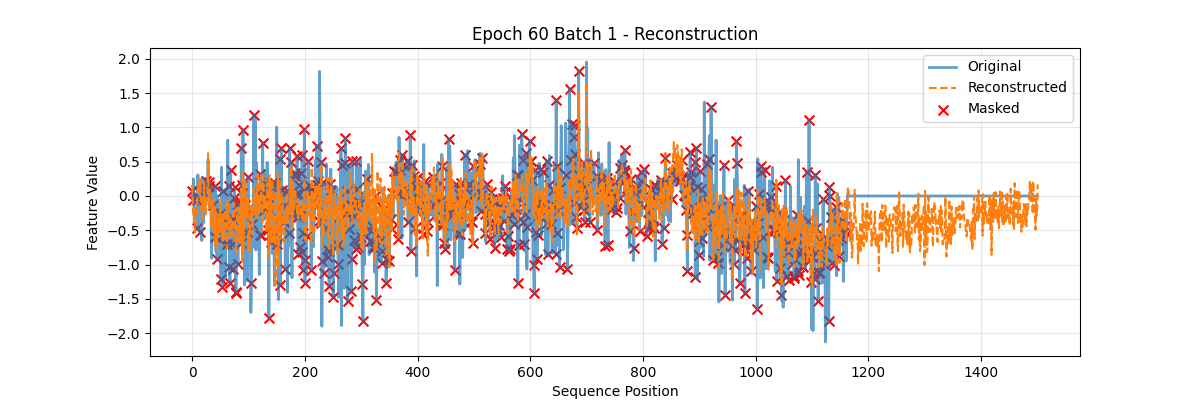
\includegraphics[width=0.8\textwidth]{imgs/epoch60_batch1.png}
		\caption{Reconstruction performance of the MAE at epoch 60. The visualization compares original embedding values (blue), reconstructed values (orange), and masked positions (red crosses). The tight alignment between original and reconstructed curves in unmasked regions demonstrates the model's capacity to learn and reproduce complex sequence-level features from incomplete data.}
		\label{fig:mae_recon}
	\end{figure}
	
	\paragraph{Feature processing strategy} Beyond standardizing individual embeddings, we also optimized the strategy for combining features from protein pairs. We explored compressing the concatenated features of a protein pair jointly, which could theoretically capture inter-protein dependencies. However, empirical tests showed this approach degraded performance, likely because extreme length disparities between paired proteins created unstable training dynamics. Our final pipeline therefore adopts a more robust strategy: compressing each protein's embedding individually and then concatenating the resulting fixed-length vectors.
	
	
	\subsection{Supervised Classification Framework}

	With standardized embeddings in hand, we framed PPI prediction as a binary classification task. To explore the feature space thoroughly, we developed a hierarchy of supervised models, moving from simple baselines to a more complex deep learning architecture.

	\paragraph{Baseline approaches} Initial benchmarks were established using simple similarity metrics (L2 distance, cosine similarity), which proved computationally efficient but insufficient for reliable prediction. A more principled baseline using logistic regression, which learns linear combinations of joint features, offered a notable improvement.

	\paragraph{Gradient boosting} To explore non-linear relationships, we implemented a gradient boosting model using XGBoost. We systematically evaluated five distinct feature-engineering strategies—from direct concatenation to element-wise operations—and applied feature scaling and early stopping to prevent overfitting.

	\paragraph{Deep neural architecture} The pinnacle of our modeling efforts is a specialized Deep Neural Network (DNN) designed to fully leverage the richness of the protein embeddings. Its architecture begins with masked average pooling to handle variable-length inputs, followed by dedicated protein encoders that transform the 960-dimensional embeddings into dense 256-dimensional representations using a sequence of linear layers, normalization, ReLU activation, and dropout (0.3).
	
	The two encoded protein vectors are then concatenated and passed to an interaction prediction module. This module consists of three fully connected layers that progressively reduce dimensionality (512 → 256 → 128 → 1), with each layer also incorporating normalization, activation, and regularization to ensure stable training and enhance generalization. The model was trained with the AdamW optimizer and a OneCycle learning rate schedule, which achieved optimal convergence with a maximum learning rate of 5e-3.
	
	\section{Experiments}
    
	\subsection{Experimental Design}

	Our evaluation utilized the benchmarking gold standard dataset (benchmarkingGS v1.0), comprising 268,499 protein pairs with UniProt identifiers, interaction labels, and complete amino acid sequences. The dataset's structure facilitates comprehensive evaluation through three distinct splits: a training set of 85,329 pairs with balanced class distribution (50.00\% positive), a similarly balanced test set (Test1) containing 24,898 pairs, and a biologically realistic test set (Test2) with 136,939 pairs exhibiting natural class imbalance (9.09\% positive interactions).

	Model development and hyperparameter optimization proceeded using a validation set of 21,333 pairs (50.00\% positive) derived from the original training data. This experimental design enables assessment of both balanced classification performance and real-world generalization under realistic class distributions. AUROC served as the primary evaluation metric, providing robust comparison across different modeling approaches.

	\subsection{Performance Analysis}

	Our results demonstrate a clear progression in predictive capability with increasing model sophistication. Simple similarity metrics achieved limited effectiveness (L2 similarity: 0.5547 AUROC), while logistic regression provided substantial improvement (0.6182 AUROC). XGBoost further enhanced performance to 0.6441 AUROC through non-linear modeling capabilities.

	Our DNN architecture delivered superior results across all evaluation scenarios. On Test1, the DNN achieved 0.7283 AUROC with 65.47\% accuracy, while maintaining robust performance on the imbalanced Test2 dataset (0.7242 AUROC). The consistent performance across both test conditions validates the model's generalization capability.

	As detailed in Table~\ref{tab:results}, our approach demonstrates substantial improvements over existing sequence-based methods, achieving 7.1\% performance gains over the best reported sequence-based model (0.6800 AUROC). This advancement underscores the effectiveness of combining ESMC-derived embeddings with specialized neural architectures for computational PPI prediction.

	\begin{table}[h]
	\caption{Comparative AUROC performance across balanced and imbalanced test datasets}
	\label{tab:results}
	\centering
	\begin{tabular}{lcc}
	\toprule
	\textbf{Method} & \textbf{Test1 AUROC} & \textbf{Test2 AUROC}\\
	\midrule
	Cosine Similarity & 0.5260 & 0.5676\\
	L2 Similarity & 0.5472 & 0.5718\\
	Logistic Regression & 0.6182 & 0.6500\\
	XGBoost & 0.6638 & 0.6660\\
	\midrule
	\multicolumn{3}{c}{\textit{Literature Baseline}}\\
	\midrule
	XGBoost & 0.62 & --\\
	Sequence-based Model & 0.68 & --\\
	\midrule
	DNN (Our Method) & \textbf{0.7283} & \textbf{0.7242}\\
	\bottomrule
	\end{tabular}
	\end{table}

	\section{Conclusion}

Our work confirms that systematically integrating ESMC-derived embeddings within a custom DNN architecture significantly advances computational PPI prediction. The resulting framework not only outperforms established baselines but also generalizes effectively across both balanced and imbalanced datasets, highlighting the power of deep learning for this task. Yet, predictive accuracy is but one measure of a model's value. The interpretability challenges common to deep learning may render such models less suitable for research where mechanistic understanding is the primary goal, reminding us that the optimal tool is dictated by the scientific question at hand.

Looking ahead, the future of PPI prediction lies in further refining these representations. Immediate opportunities include developing embedding strategies that better preserve the structural information lost in compression. A more transformative step, however, will be end-to-end fine-tuning, directly optimizing the protein language model for interaction discovery. The convergence of large-scale protein modeling with specialized architectures marks a significant step forward, promising more powerful tools to map the interactome and unravel the molecular basis of life.

	\bibliographystyle{plain}
	\bibliography{references}
	
	%%%%%%%%%%%%%%%%%%%%%%%%%%%%%%%%%%%%%%%%%%%%%%%%%%%%%%%%%%%%
	
	
\end{document}